% documentclass options:
\documentclass[11pt,
  a4paper,
  parskip=half, % This is some extra vertical space between paragraphs, the suggestion is 2cm which is really ugly, so we use what koma script gives us
  % you can also set it to full for even more space. But there is a bad tex style decision: parskip also changes the spacing between listitems such as
  % enumerate and itemize. For this purpose we include the enumitem package and set itemsep=.5em, of course you can change this
  BCOR=10mm, % BCOR is binding correction
  english,
  % if you'd rather have a one sided thesis, add `oneside' to the documentclass
  oneside,
  % ngerman is needed for hyphenation if the thesis contains parts written in German, switch order with english if you write mainly in English.
  % Remember to change order in the babel package (below) as well.
  % Last language is the preferred one.
  ngerman]{scrbook}
\usepackage[english, ngerman]{babel} % If you write mainly in English change order to ngerman, english. Also change that in the documentclass options above.
% Include of titling must happen before \title etc.
% that's why it's not in setup.tex
\usepackage{titling}
\title{Modellrekonstruktion anhand der Covid-19-Daten der deutschen Landkreise}
\author{Leander Marius Bürkin}

% Change to your first examiner
% The ~ enables non sentence spacing after a period
\newcommand{\firstexaminer}{Dr.~Andreas Greiner}
% Change to your second examiner, some undergraduate studies don't have a second examiner
% in this case just comment out the following line
\newcommand{\secondexaminer}{Prof.~Dr.~Moritz Mathias Diehl}
% Change to your adivers
\newcommand{\advisers}{Dr.~Andreas Greiner}

% include all packages and define commands in setup.tex

%------------------------------------------------------------------------------
%       package includes
%------------------------------------------------------------------------------
    % font encoding is set up for pdflatex, for other environments see
    % http://tex.stackexchange.com/questions/44694/fontenc-vs-inputenc
    \usepackage[T1]{fontenc}  % 8-bit fonts, improves handling of hyphenations
    \usepackage[utf8]{inputenc}
    % provides `old' commands for table of contents. Eases the ability to switch
    % between book and scrbook
    \usepackage{scrhack}

    % ------------------- layout, default -------------------
    % adjust the style of float's captions, separated from text to improve readabilty
    \usepackage[labelfont=bf, labelsep=colon, format=hang, textfont=singlespacing]{caption}
    % With format = hang your caption will look like this:
    % Figure 1: Lorem ipsum dolor sit amet,
    %           consectetuer adipiscing elit.
    %           Ut purus elit, vestibulum
    % If you instead want
    % Figure 1: Lorem ipsum dolor sit amet,
    % consectetuer adipiscing elit. Ut purus
    % elit, vestibulum
    % change to format=plain
    \usepackage{chngcntr}  % continuous numbering of figures/tables over chapters
    \counterwithout{equation}{chapter}
    \counterwithout{figure}{chapter}
    \counterwithout{table}{chapter}

    % Uncomment the following line if you switch from scrbook to book
    % and comment the setkomafont line
    %\usepackage{titlesec}  % remove "Chapter" from the chapter title
    %\titleformat{\chapter}[hang]{\bfseries\huge}{\thechapter}{2pc}{\huge}
    \setkomafont{chapter}{\normalfont\bfseries\huge}

    \usepackage{setspace}  % Line spacing
    \onehalfspacing
    % \doublespacing  % uncomment for double spacing, e.g. for annotations in correction

    % ------------------- functional, default-------------------
    \usepackage[dvipsnames]{xcolor}  % more colors
    \usepackage{array}  % custom format per column in table - needed on the title page
    \usepackage{graphicx}  % include graphics
    \usepackage{subfig}  % divide figure, e.g. 1(a), 1(b)...
    \usepackage{amsmath}  % |
    \usepackage{amsthm}   % | math, bmatrix etc
    \usepackage{amsfonts} % |
    \usepackage{calc}  % calculate within LaTeX
    \usepackage[unicode=true,bookmarks=true,bookmarksnumbered=true,
                bookmarksopen=true,bookmarksopenlevel=1,breaklinks=false,
                pdfborder={0 0 0},backref=false,colorlinks=false]{hyperref}
    \usepackage{etoolbox} % if-else commands


    %==========================================
    % You might not need the following packages, I only included them as they
    % are needed for the example floats
    % ------------------- functional, custom -------------------
    \usepackage{algorithm2e,algpseudocode}
    \usepackage{bm}  % bold greek variables (boldmath)
    \usepackage{tikz}
    \usetikzlibrary{positioning}  % use: above left of, etc
    
    % Required for the ToDo list.
    \usepackage{ifthen}

    % Improves general appearance of the text
    \usepackage[protrusion=true,expansion=true, kerning]{microtype}
    \usepackage{enumitem}
    % Nicer font for pdf rendering.
    %\usepackage{lmodern}
    
    % For nicer looking tables.
    \usepackage{booktabs}

    % You don't need this, just for demonstration of a longer caption.
    \usepackage{lipsum}

%------------------------------------------------------------------------------
%       (re)new commands / settings
%------------------------------------------------------------------------------
    % ----------------- referencing ----------------
    \newcommand{\secref}[1]{Sektion~\ref{#1}}
    \newcommand{\chapref}[1]{Kapitel~\ref{#1}}
    \renewcommand{\eqref}[1]{Gleichung~(\ref{#1})}
    \newcommand{\figref}[1]{Abbildung~\ref{#1}}
    \newcommand{\tabref}[1]{Tabelle~\ref{#1}}

    % ------------------- colors -------------------
    \definecolor{darkgreen}{rgb}{0.0, 0.5, 0.0}
    % Colors of the Albert Ludwigs University as in
    % https://www.zuv.uni-freiburg.de/service/cd/cd-manual/farbwelt
    \definecolor{UniBlue}{RGB}{0, 74, 153}
    \definecolor{UniRed}{RGB}{193, 0, 42}
    \definecolor{UniGrey}{RGB}{154, 155, 156}


    % ------------------- layout -------------------
    % prevents floating objects from being placed ahead of their section
    \let\mySection\section\renewcommand{\section}{\suppressfloats[t]\mySection}
    \let\mySubSection\subsection\renewcommand{\subsection}{\suppressfloats[t]\mySubSection}



    % ------------------- math formatting commands -------------------
    % define vectors to be bold instead of using an arrow
    \renewcommand{\vec}[1]{\mathbf{#1}}
    \newcommand{\mat}[1]{\mathbf{#1}}
    % tag equation with name
    \newcommand{\eqname}[1]{\tag*{#1}}


    % ------------------- pdf settings -------------------
    % ADAPT THIS
    \hypersetup{pdftitle={\thetitle},
                pdfauthor={\theauthor},
                pdfsubject={Undergraduate thesis at the Albert Ludwig University of Freiburg},
                pdfkeywords={simulation, corona, covid19, model reconstruction, diffusion, spreading},
                pdfpagelayout=OneColumn, pdfnewwindow=true, pdfstartview=XYZ, plainpages=false}


    %==========================================
    % You might not need the following commands, I only included them as they
    % are needed for the example floats

    % ------------------- Tikz styles -------------------
    \tikzset{>=latex}  % arrow style


    % ------------------- algorithm ---------------------
    % Command to align comments in algorithm
    \newcommand{\alignedComment}[1]{\Comment{\parbox[t]{.35\linewidth}{#1}}}
    % define a foreach command in algorithms
    \algnewcommand\algorithmicforeach{\textbf{foreach}}
    \algdef{S}[FOR]{ForEach}[1]{\algorithmicforeach\ #1\ \algorithmicdo}

    % line spacing should be 1.5
    \renewcommand{\baselinestretch}{1.5}

    % set distance between items in a list, for more details see the
    % enumitem package: https://www.ctan.org/pkg/enumitem
    \setlist{itemsep=.5em}
    
    % use ra in your tables to increase the space between rows
    % 1.3 should be fine
    \newcommand{\ra}[1]{\renewcommand{\arraystretch}{#1}}

	% ToDo counters
	\usepackage{ifthen} %für whiledo-Schleife
	\newcounter{todos}
	\setcounter{todos}{0}
	\newcounter{extends}
	\setcounter{extends}{0}
	\newcounter{drafts}
	\setcounter{drafts}{0}

	% ------------------- marker commands -------------------
    % ToDo command
    \newcommand{\todo}[1]{\textbf{\textcolor{red}{(TODO: #1)}}\refstepcounter{todos}\label{todo \thetodos}}
	\newcommand{\extend}[1]{\textbf{\textcolor{darkgreen}{(EXTEND: #1)}}\refstepcounter{extends}\label{extend \theextends}}
	% Lighter color to note down quick drafts
	\newcommand{\draft}[1]{\textbf{\textcolor{NavyBlue}{(DRAFT: #1)}}\refstepcounter{drafts}\label{draft \thedrafts}}
	
	% microtype with lmodern, see https://tex.stackexchange.com/questions/75305/microtype-warning-with-lmodern-package-and-koma-script
	%\DeclareMicrotypeAlias{lmss}{cmr}
	
	\renewcommand{\listalgorithmcfname}{Algorithmenverzeichnis}
	\renewcommand{\algorithmcfname}{Algorithmus}
	
	
	
%  ------------------- my own packages -------------------

    
    % to add biber/biblatex handling the references
    \usepackage[backend=biber]{biblatex}
    \addbibresource{References/Refs_Grundlagen_und_Stand_der_Forschung.bib}
    \addbibresource{References/Refs_Motivation.bib}
    \addbibresource{References/Refs_Zitatseite.bib}
    \usepackage{csquotes}
    
    % to prevent underfull/overfull hbox
    \usepackage{parskip}

    % to pack content into multiple cells of a table
    \usepackage{multirow}

\begin{document}
    \pagestyle{empty} % no header and no page number
    % disable hyper links to remove warning "destination with same identifier"
    % this means within this section nothing can be referenced with a hyperlink
    \hypersetup{pageanchor=false}

    % enable/disable, depending on your chosen language
    \begin{titlepage}
\begin{center}
\ \\
\newcommand{\HorizontalLine}{\rule{\linewidth}{0.3mm}}
{\large Bachelorarbeit}\\[-0.5cm]
\HorizontalLine \\[0.4cm]
{ \huge \bfseries \thetitle }
\HorizontalLine \\[0.7cm]

{\huge \theauthor} \\[1cm]
\begin{tabular}[hc]{>{\large}l >{\Large}l}
  Gutachter: & \secondexaminer\\
  Betreuer: & \advisers\\[1cm]
\end{tabular}
\setlength{\fboxrule}{2pt}
\setlength{\fboxsep}{0pt}
\fbox{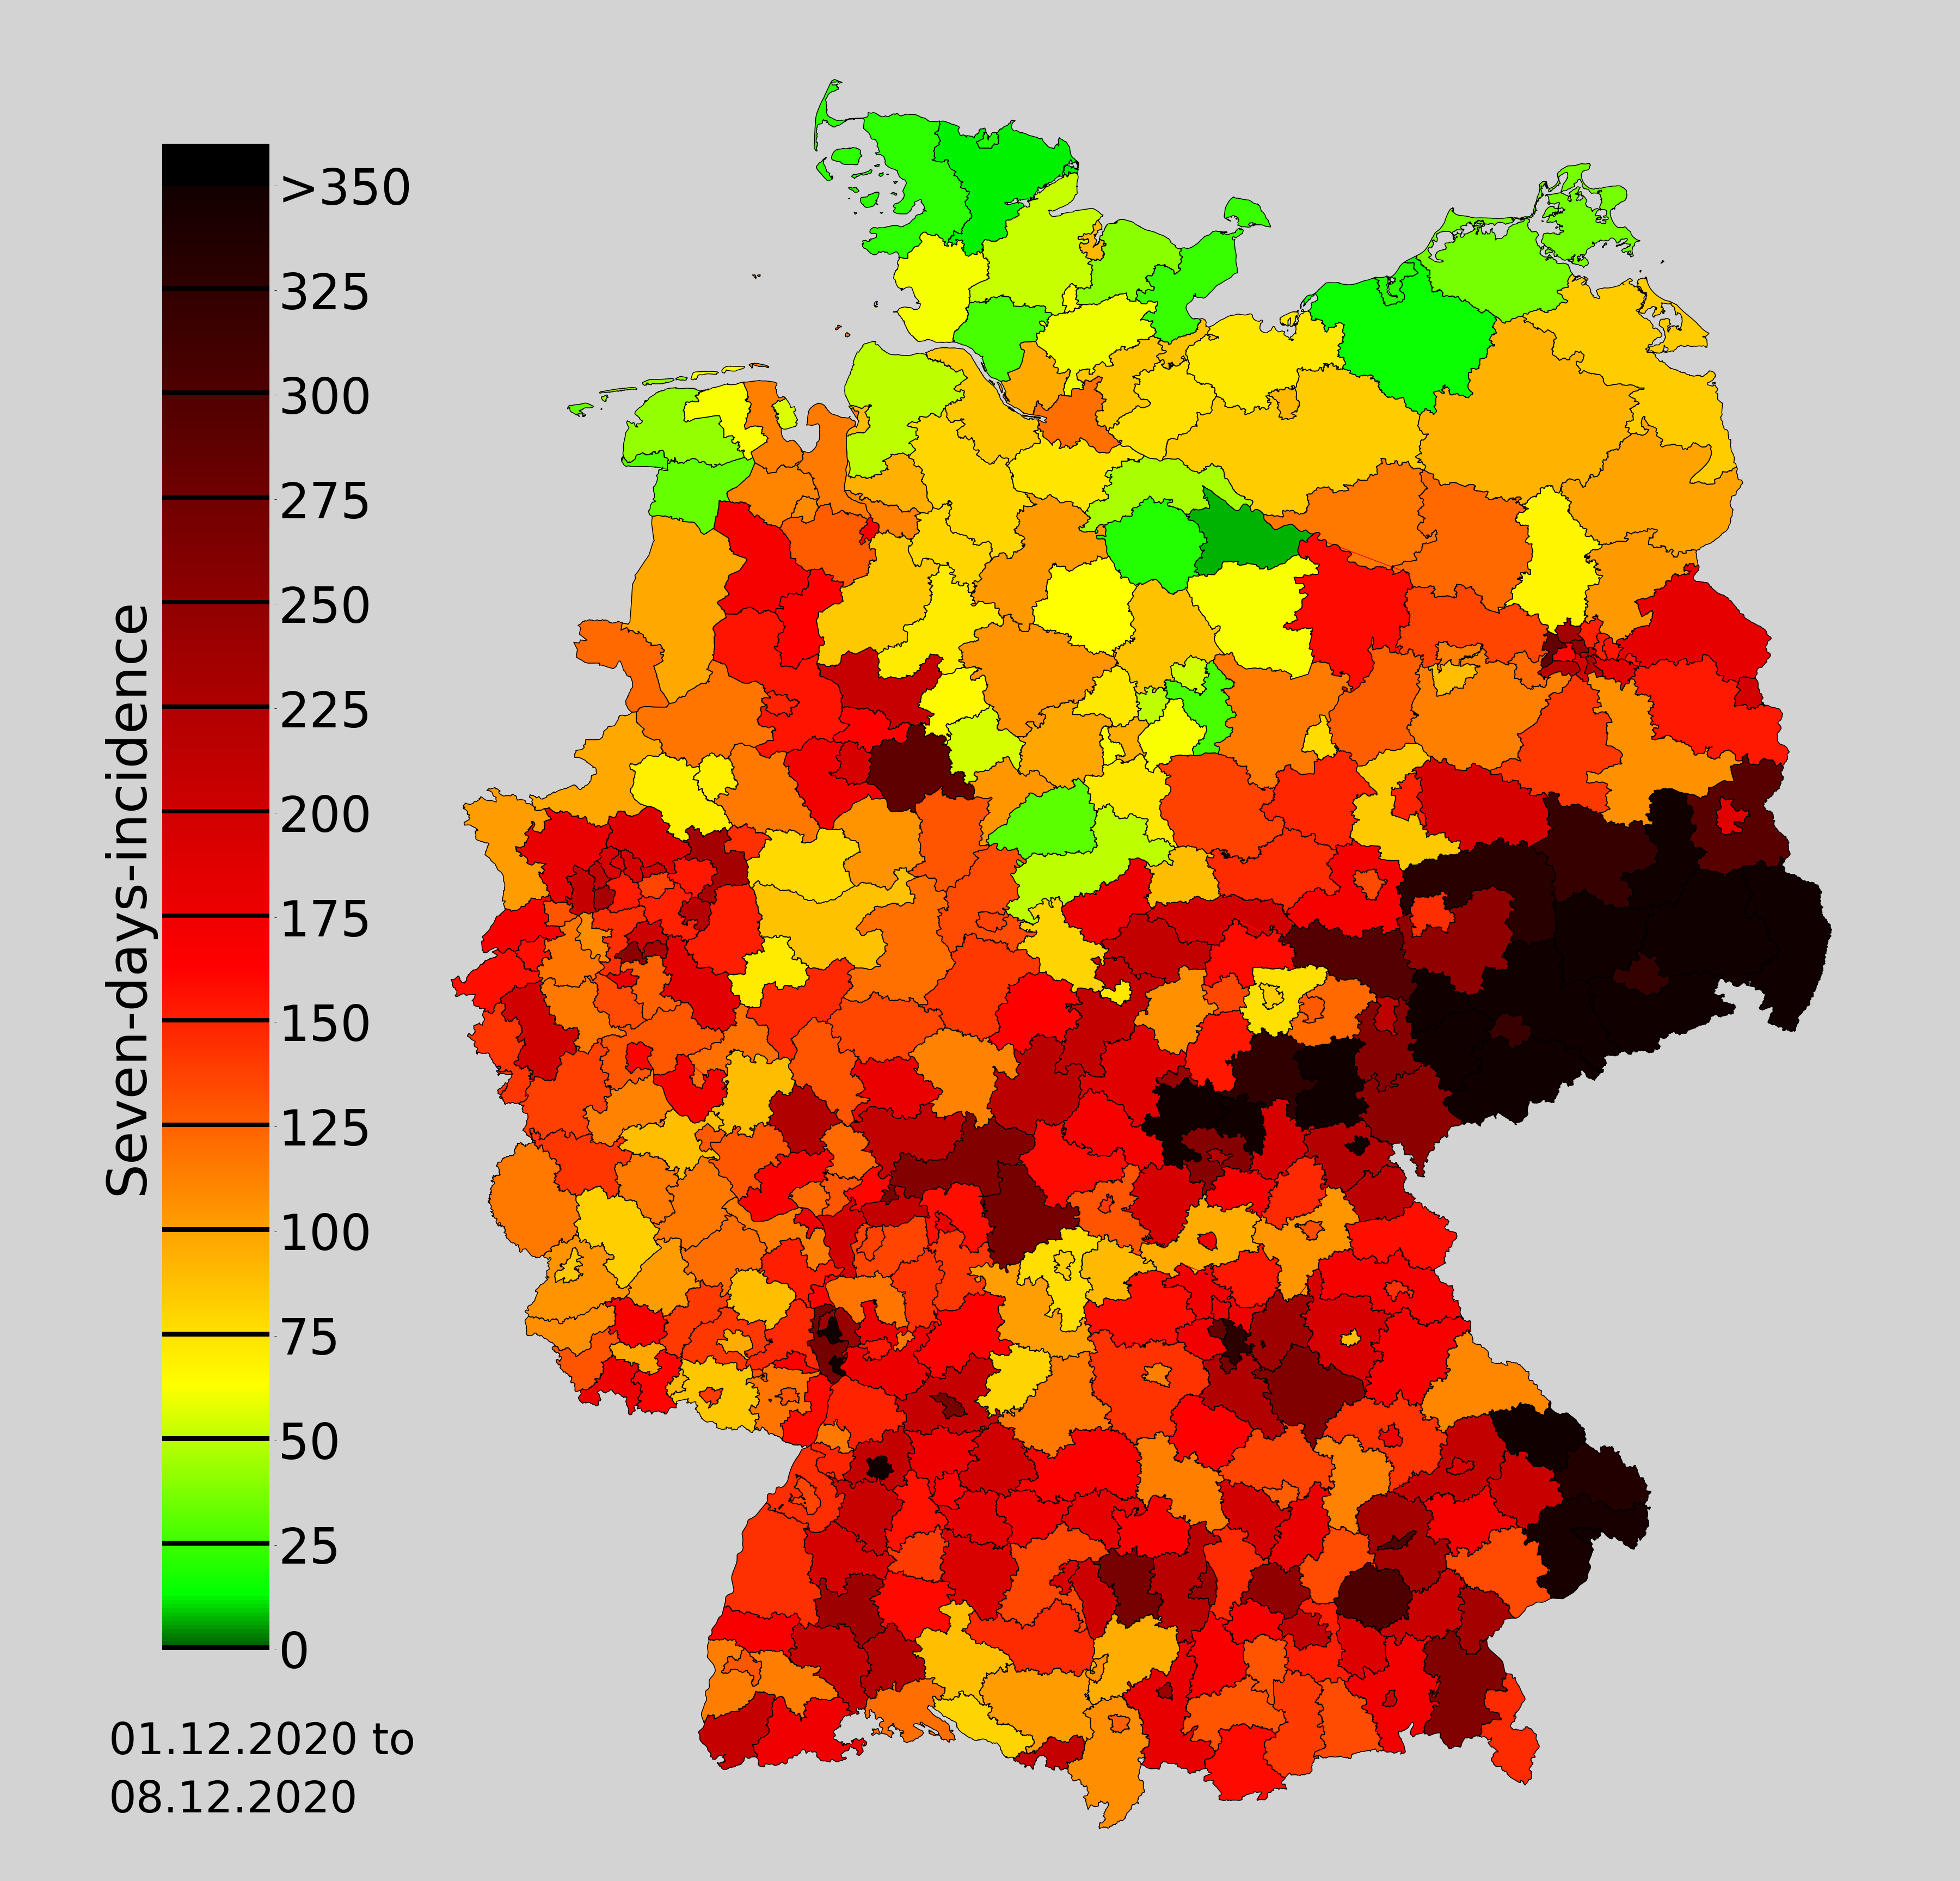
\includegraphics[width=0.6\textwidth]{figures/vor_dem_Inhaltsverzeichniss/282lightgrey.png}}
\\[1cm]
Lehrstuhl für Simulation\\[-0.25cm]
Institut für Mikrosystemtechnik - IMTEK\\[-0.25cm]
Albert-Ludwigs-Universität, Freiburg im Breisgau
\end{center}
\end{titlepage}

\thispagestyle{empty}
\ \vfill \ \\
\
\textbf{Bearbeitungszeit} \todo{change date}           \smallskip{} \\
05.\,07.\,2016 -- 05.\,10.\,2016    \bigskip{} \\
\
\textbf{Gutachter}                  \smallskip{} \\
\firstexaminer                      \bigskip{} \\
\
% If there is a second examiner include it
\textbf{Zweitgutachter}             \smallskip{} \\
\secondexaminer                     \bigskip{} \\
\
\textbf{Betreuer}                   \smallskip{} \\
\advisers

    \pagestyle{plain} % remove chapter name from top, page number at the bottom
    % use \pagestyle{headings} for having the chapter on top of the pages
    % if you wang a more fancy header use \usepackage[automark,headsepline]{scrlayer-scrpage}
    % and read about it in the KOMA script documentation, https://www.ctan.org/pkg/koma-script
    \frontmatter  % roman page numbers
    \chapter*{Erklärung}
Hiermit erkläre ich, dass ich diese Abschlussarbeit selbständig verfasst habe, keine anderen als die angegebenen Quellen/Hilfsmittel verwendet habe und alle Stellen, die wörtlich oder sinngemäß aus veröffentlichten Schriften entnommen wurden, als solche kenntlich gemacht habe. Darüber hinaus erkläre ich, dass diese Abschlussarbeit nicht, auch nicht auszugsweise, bereits für eine andere Prüfung angefertigt wurde.
\\[3\normalbaselineskip]
\begin{tabular}{p{\textwidth/2} l}
  \rule{\textwidth/3}{0.4pt}   &   \rule{\textwidth/3}{0.4pt} \\
  Ort, Datum                  &   Unterschrift
\end{tabular}

    \chapter*{Abstract}
\chapter*{Kurzfassung}
Die Jahre 2020 und 2021 waren vom Coronavirus und der einhergehenden Unsicherheit geprägt - Wie verbreitet sich das Virus? Wie schnell entstehen Hotspots? Ganz allgemein: Ist die Ausbreitung irgendwie einfach quantifizierbar?

Ein Versuch, diese Fragen zu beantworten und die gegebenen Corona-Daten zusammenzufassen, ist in dieser Arbeit beschrieben. Im speziellen werden die Daten, welche das Robert Koch-Institut über ArcGIS zur Verfügung stellt, mit mathematischen Formeln der Diffusion analysiert.


Zu jedem deutschen Landkreis liefert das Robert Koch-Institut die akkumulierten Infektionszahlen seit dem 01.03.2020, die Fläche, die Position sowie die von den statistischen Landesämtern geschätzte Einwohnerzahle am 31.12.2019, welche in Deutschland zur Berechnung der 7-Tage-Inzidenz (Neuansteckungen pro 100.000 Einwohnern in 7 Tagen) benutzt wird.


Aus diesen Daten lässt sich der Verlauf folgender Größen darstellen:
\begin{itemize}
    \item Akkumulierte Fallzahlen eines Landkreises
    \item Das Verhälniss von Ansteckbaren (S), Infizierten (I) und aus dem Infektionsgeschehen entfernten Personen (R bzw. R und D, wenn Tote gesondert aufgeführt werden) - dies entspricht dem SIR-Modell
    \item 7-Tage-Inzidenz eines Landkreises
    \item 7-Tage-Inzidenzen aller Landkreise
    \item 7-Tage-Inzidenzen aller Landkreise im Vergleich zur Bevölkerungsdichte des Landkreises
    \todo{checken, ob alle hier aufgeführten Abbildung in der finalen Arbeit stecken.}
\end{itemize}

\todo{Das folgende wurde Aus Motivation hierher verschoben, bitte einpflegen}

Ziel dieser Arbeit ist es, aus allen vorliegenden COVID-19 Daten der deutschen Landkreise ein leicht zugängliches Bild zu erzeugen, welches schwer vorstellbare Prozesse visualisiert und mit einfachsten Mitteln der Mathematik einige mögliche Abhängigkeiten nachzuprüfen.

\todo{Ergebnisse in Zusammenfassung hinzufügen}
\todo{Abstract übersetzen}
\newpage
    \vspace*{15pt}
\begin{center}
    \huge{\textbf{
    \textit{Those who cannot remember the past\\ are condemned to repeat it.}}}
    \large{- George Santayana \autocite{history-quoteSantayana}}
\end{center}
\vspace*{65pt}
\begin{figure}[h]
    \centering
    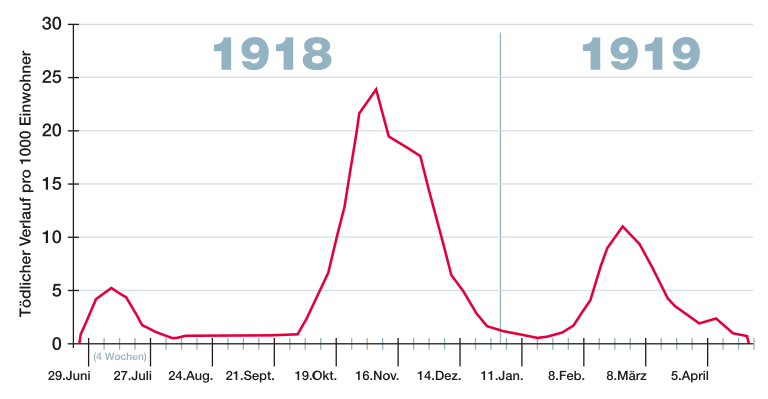
\includegraphics[width=0.71\textwidth]{figures/Spanische_Grippe_1918_1919_GB.svg.png}
    \caption{Die drei Wellen der \glqq{}Spanischen Grippe\grqq{} in Großbritannien, wöchentliche kombinierte Grippe- und Lungenentzündungssterblichkeit von Juni 1918 bis Mai 1919. \autocite{spanischflu}}
    \label{fig:spanishflu}
\end{figure}

\begin{figure}[h]
    \centering
    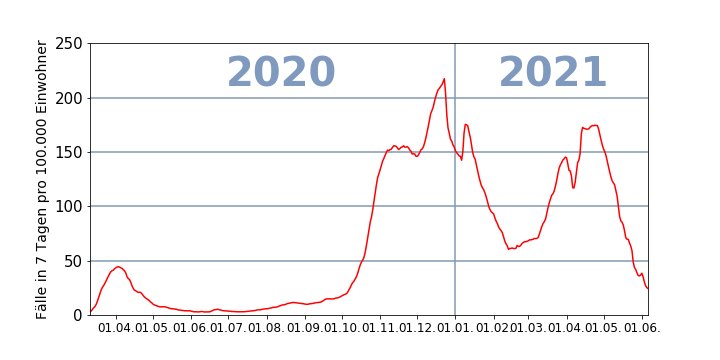
\includegraphics[width=0.76\textwidth]{figures/Inzidenz Deutschland.png}
    \caption{Die drei Wellen der COVID-19-Pandemie in Deutschland, dargestellt durch die sieben Tage Inzidenz jeden Tages über den Zeitraum vom 01.03.2020 bis 05.06.2021.}
    \label{fig:germany_incidence}
\end{figure}
    \tableofcontents
    \listoffigures
    \listoftables
    \listofalgorithms
    \hypersetup{pageanchor=true}  % re-enable hyperlinking

    \mainmatter  % Arabic page numbers
    \chapter{Motivation}\label{chap:Motivation}
Viele große Zivilisationen hatten bereits mit Pandemien ähnlich zur aktuellen COVID-19 Pandemie zu kämpfen.\\
Schon aus dem Alten Rom haben wir Zeugnisse der Antoninischen Pest im zweiten Jahrhundert nach Christus: Vermutlich ein Pocken Ausbruch, dessen 7-10 Millionen Tote das Römische Reich destabilisierten (\autocite{RomPest}, S. 255).
Im Mittelalter kamen 200 Millionen Menschen durch die Pest um \autocite{PestMittelalter}.
Die Armeen des ersten Weltkriegs wurden ebenfalls durch die Spanische Grippe geschwächt: Sie forderte circa 100 Millionen Opfer weltweit \autocite{SpanischeGrippe}.

Doch nicht nur in den dicht besiedelten Gebieten des Mittelmeerraums und des Nahen Ostens sorgten Pandemien für Instabilität: Sie sind seit jeher ein weltweites Problem und können durch Reisen ausgleöst oder stark verstärkt werden.\\
Nach 1707 starben innerhalb von zwei Jahren circa 18.000 der 50.000 Einwohner Islands an Pocken (\autocite{americaPandemics}, Seite 325 Zeile 20ff). Vieles spricht für einen ähnlich vernichtenden Pockenausbruch bei den Azteken, den Inka und den andere Völkern der Neuen Welt \autocite{americaPandemics}.

Über diese vergangenen Pandemien wissen wir recht wenig, da sie beispielsweise durch den Zorn Gottes erklärt wurden(\autocite{americaPandemics}, Seite 324 Zeile 7) oder die genannten Zahlen eher die Gefühle der Zeitzeugen widerspiegeln als statistische Daten zu liefern (\autocite{americaPandemics}, Seite 324 Zeile 20ffff). Mit dem heutigen Stand der Datenerfassung und -übermittlung lässt sich die COVID-19 Pandemie sehr viel einfacher untersuchen als ihre Vorgänger.

um derartige Todeswellen zu vermeiden und einer Zivilisation Stabilität zu bieten, ist es wichtig, diese einschneidenden Ereignisse mit verschiedensten Ansätzen zu untersuchen. 

Die meisten von uns haben genau diese Zahlen des Robert-Koch-Instituts oder der Weltgesundheitsorganisation beobachtet und versucht zu verstehen, wie man sich morgen zu Verhalten hat. Viele Hypothesen wurden aufgestellt und jede*r musste sich auf einmal mit Epidemiologie beschäftigen, wobei wir meist nur ein Puzzleteil vor Augen hatten.

Trotz immenser Bemühungen brachte die aktuelle COVID-19 Pandemie unser Gesundheitssystem an seine Grenzen: Kleinere Krankenhäuser wurden schnell überwältigt, wenn der Bedarf an Beatmungsgeräten größer wurde als ihre Kapazitäten.

Daher soll diese Arbeit das gesellschaftliche Verständniss für zukünftigen Pandemien schärfen, damit die Ausbreitung zukünfitger Erreger verlangsamt wird und ein Kollaps des Gesundheitssystems oder gar der gesamten Zivilisation verhindert werden kann.

    \chapter{Grundlagen und Stand der Forschung}\label{chap:Grundlagen und Stand der Forschung}
\section{Susceptible-Infectious-Removed Modell}
Ein Weg zur Beschreibung der Pandemie bietet das SIR Modell \autocite{SIR}. Dieses Modell teilt die Mitglieder einer Menschengruppe in eine der drei folgenden Kategorie ein und ermöglicht es, die zeitliche Entwicklung einer Pandemie übersichtlich darzustellen:
\begin{itemize}
    \item \glqq{}susceptible\grqq{}: Menschen, welche angesteckt werden können.
    \item \glqq{}infectious\grqq{}: Infizierte Menschen, welche weitere Menschen anstecken können.
    \item \glqq{}recovered\grqq{}: Menschen, welche in die Kategorie \glqq{}infectious\grqq{} fielen und\\
    nun immun gegen die Krankheit sind. (Hierzu zählen auch Verstorbene)
\end{itemize}
Hierbei werden die Neuansteckungen ausgehend von einem infizierten Menschen mit der Reproduktionszahl $R$ beschrieben. Formal ist die Reproduktionszahl $R$ definiert durch die durchschnittliche Anzahl an infizierten Menschen pro Fall \autocite{ReZahl}.
%weitere Erklärung von R_0 siehe Fabians erste Einleitungsseite




\section{Korrelationsanalyse mithilfe einer Faltung}\label{sec:Korrelationsanalyse}

    \chapter{Vorgehensweise}\label{chap:Vorgehensweise}
Diese Bachelorarbeit basiert auf den Vorleistungen des Bachelorprojekts von Leander Marius Bürkin.

\section{Bachelorprojekt von Leander Bürkin}
Ziel dieses Bachelorprojekts war eine Reihe an Deutschlandkarten in einem Video zusammenzufassen, welches die Ausbreitung der COVID-19 Pandemie in Deutschland vom ersten März 2020 bis zum letzten Tag, für den die API des RKIs Daten liefert, darstellt.

\subsection{Ergebniss}
Das fertige Videos ist verfügbar unter \todo{Video verlinken}.\\
Die vom Program ausgegebene Reihe an Bilddateien wurde mithilfe des Windows Video Editors erstellt.
\\
\todo{sieben Tages Inzidenz erklären}
Die Farbe jedes Landkreises repräsentiert die sieben Tage Inzidenz des Landkreises gemäß der Legende.\\
Eine Reihe von Histogramen auf der rechten Seite zeigt die Verteilung der sieben Tage Inzidenzen alles deutschen Landkreise. Ein Histogram besteht aus 15 Säulen, wobei jede Säule einen Inzidenzbereich von 25 abdeckt. Die letzte Säule enthält zusätzlich alle sieben Tages Inzidenzen größer 350 Fälle pro sieben Tage und 100.000 Einwohner. Die Höhe der Säule entspricht jeweils der Anzahl an Landkreisen mit einer sieben Tages Inzidenz im angegebenen Bereich.

\subsection{Programmdateien}
Im Anhang finden sich die drei Programmdateien, aus denen sich sich das Programm zusammensetzt: \todo{link project files}


Die Dateien haben eine hierarchische Struktur:\\
Die Datei \glqq{}plot\_data.ipynb\grqq{} führt die Datei \glqq{}get\_data.ipynb\grqq{} aus,
welche wiederum die Datei \glqq{}get\_geographical\_data\_of\_german\_counties.ipynb\grqq{} ausführt.

Die Datei \glqq{}plot\_data.ipynb\grqq{} speichert die Grafiken schlussendlich\\
in den Ordner \glqq{}media\grqq{}.

Die Datei \glqq{}get\_data.ipynb\grqq{} konvertiert \glqq{}unpolierte\grqq{} Daten zu \glqq{}polierten\grqq{} Daten.

\glqq{}Unpolierte\grqq{} Daten sind rohe Daten direkt vom RKI oder ein Backup von diesen Daten.

Daten, die rudimentär auf Vollständigkeit überprüft wurde und bei welcher überflüssige Informationen entfernt wurde, werden \glqq{}polierte\grqq{} Daten genannt.\\
Die Datei \glqq{}get\_geographical\_data\_of\_german\_counties.ipynb\grqq{} ist ein ausgelagerter Teil von der Datei \glqq{}get\_data.ipynb\grqq{}, welcher die Informationen über die Form und die Lage der deutschen Landkreise beschafft. Dieser Vorgang nimmt überdurchschnittlich viel Platz ein, da die Form von circa 100 Landkreisen von Hand überprüft werden muss.

\subsection{Daten}
\subsubsection{Format und Aufteilung der Daten}
Die Daten liegen in einer Kombination aus Python Dictionaries und Python Listen vor. Ein Dictionary ist dadurch charakterisiert, dass man über den Namen eines Elements (der \glqq{}Key\grqq{}) das Element bekommt, ähnlich der Adresse bei einem Haus. Listen sind dadurch charakterisiert, dass sie Elemente in einer fixen Reihenfolge enthalten und sich diese durch ihren Index leicht ausfindbar machen. So sind beispielsweise die Anzahl der COVID-19 Fälle der einzelnen Tage chronologisch in einer Liste gespeichert, sodass man daraus direkt eine Abbildung erstellen kann.\ \\
Die Programmdateien erstellen drei verschiedene Dictionaries, welche (in untergeordneten Dictionaries und Listen) alle Daten enthalten:
\begin{itemize}
    \item covid19
    \item counties\_geography
    \item non\_county\_specific\_data
\end{itemize}

\textbf{covid19}\\
Das Dictionary covid19 speichert die COVID-19 Fälle jedes deutschen Landkreises und die daraus berechnete sieben Tages Inzidenz.

Mit dem Gemeindeschlüssel eines Landkreises als Key und dem zusätzlichen Key \glqq{}cases\grqq{} erhält man die akkumulierte Anzahl an COVID-19 Fällen pro Tag des Landkreises als Liste.

Mit dem Gemeindeschlüssel eines Landkreises als Key und dem Key \glqq{}incidences\grqq{} erhält man die sieben Tages Inzidenz pro Tag des Landkreises als Liste.

Beide Listen enthalten für jeden Tag seit dem 01.03.2020 bis zu dem Tag der aktuellsten Daten jeweils einen Eintrag.

Die Anzahl an COVID-19 Fällen pro Tag stamt aus dem \glqq{}COVID-19 Datenhub\grqq{} (https://npgeo-corona-npgeo-de.hub.arcgis.com/). Die sieben Tages Inzidenz wurde aus den Daten vom COVID-19 Datenhub berechnet.

\textbf{counties\_geography}\\
Das Dictionary counties\_geography enthält zu jedem Landkreis ein Dictionary mit den folgenden Elemente:
\begin{itemize}
    \item[name:] Der Name des Landkreises
    \item[population:] Die Einwohnerzahl des Landkreis aus einer offiziellen Schätzung (nähere Informationen finden sich im COVID-19 Datenhub). Diese Zahlen werden auch für die offizielle Berechnung der sieben Tages Inzidenz verwendet.
    \item[area\_in\_m2:] Die Fläche des Landkreises in Quadratmetern
    \item[geometry:] Die Form des Landkreises in einer für die Darstellung angepassten Form
    \item[raw\_geometry:] Die Form des Landkreises in der originalen Form
    \item[population\_density:] Die Bevölkerungsdichte des Landkreises, berechnet aus der Fläche des Landkreises und seiner Einwohnerzahl
\end{itemize}
Außer die Bevölkerungsdichte, welche berechnet wird, und die angepassten Formen der Landkreise, welche aus den origialen Formen generiert werden, stammen alle Daten direkt aus dem \glqq{}COVID-19 Datenhub\grqq{} (https://npgeo-corona-npgeo-de.hub.arcgis.com/).

\textbf{non\_county\_specific\_data}
Das Dictionary non\_county\_specific\_data enthält die folgenden Elemente:
\begin{itemize}
    \item[unixtime:] Die Unixzeit, wie sie vom COVID-19 Datenhub zur Verfügung gestellt wird: Die Zahl der Millisekunden seit dem 01.01.1970 00:00 Uhr UTC. Die Zahl der COVID-19 Fälle und die sieben Tages Inzidenz eines entsprechenden Tages befinden sich an der selben Stelle in Ihrer jeweiligen Liste, wie der Tag in dieser Liste.
    \item[states:] Die Name und Nummern der deutschen Bundesländer. Die ersten beiden oder die erste Zahl des Gemeindeschlüssel eines Landkreises repräsentiert das Bundesland, in welchem der Landkreis liegt.
    \item[highest\_case\_number:] Die höchste akkumulierte Fallzahl unter allen Landkreisen.
    \item[lowest\_case\_number:] Die niedrigste akkumulierte Fallzahl unter allen Landkreisen.
    \item[highest\_incidence:] Die höchste sieben Tages Inzidenz eines Tages unter allen Landkreisen.
    \item[lowest\_incidence:] Die niedrigste sieben Tages Inzidenz eines Tages unter allen Landkreisen.
    \item[UTC:] Die Unixzeit konvertiert in die Koordinierte Weltzeit \glqq{}DD.MM.YYYY\grqq{}.
    \item[UTC+7days:] Die Liste der Zeiten gespeichert in UTC plus sieben Tage vor dem erstem Datum in der Liste, um den Zeitraum der sieben Tages Inzidenz der ersten sieben Tage darstellen zu können: die hierfür verwendeten Zeiträume beginnen jeweils vor dem ersten hier dokumentierten Fall.
\end{itemize}
Die Unixzeit, die Namen und die Nummern der Bundesländer stammen aus dem \glqq{}COVID-19 Datenhub\grqq{} (https://npgeo-corona-npgeo-de.hub.arcgis.com/). Alle anderen Informationen wurden gesammelt oder berechnet.
\begin{figure}
    \centering
    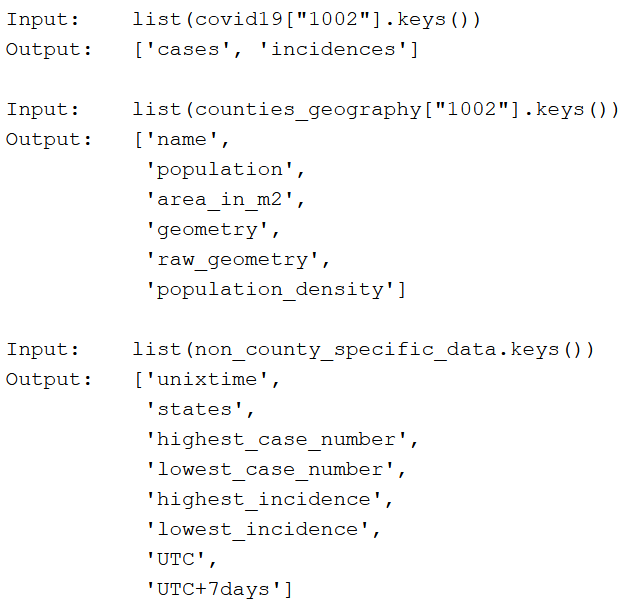
\includegraphics[width=0.9\textwidth]{figures/Dictionarys Bachelorprojekt.png}
    \caption{
    Die Dictionaries non\_county\_specific\_data, counties\_geography und covid19 mit ihren jeweiligen Schlüsseln.
    Für die Dictionaries covid19 und counties\_geography wurde jeweils der Landkreis Kiel (Gemeindeschlüssel 1002) zur Veranschaulichung verwendet.}
    \label{fig:my_label}
\end{figure}

\subsubsection{Datenquellen - Ursprung und Abspeicherung}
Das Bachelorprojekt verwendet Informationen zur COVID-19 Pandemie und den geographischen Daten von 412 deutschen Landkreisen. Alle Daten stammen aus dem \glqq{}COVID-19 Datenhub\grqq{} (https://npgeo-corona-npgeo-de.hub.arcgis.com/) oder wurden aus den daher stammenden Daten generiert. Diese Datenquelle wurde gewählt, weil sie vom Robert-Koch-Institut (RKI, www.rki.de) und dem deutschen Staat referenziert wird.

Die Daten sind in drei verschiedenen Formen gespeichert:
\begin{itemize}
    \item Als originale Daten auf dem Server des RKIs, erreichbar durch eine sogenannte API.
    \item Als unpolierte Daten auf der Maschine, welche das Program ausführt, als Backup, wenn die API nicht erreichbar ist.
    \item Als polierte Daten auf der Maschine, welche das Program ausführt, für den sofortigen Gebrauch.
\end{itemize}
\todo{Vergleiche mit https://www.rki.de/DE/Content/Infekt/EpidBull/Archiv/2020/Ausgaben/17_20.pdf?__blob=publicationFile  }
    \chapter{Ergebnisse}\label{chap:Ergebnisse}

    \chapter{Diskussion}\label{chap:Diskussion}
    \chapter{Zusammenfassung}\label{chap:Zusammenfassun}
    \chapter{Danksagung}
Vielen herzlichen Dank den zahlreichen Helfern, welche mich mental und inhaltlich unterstützt haben!

Zuallererst danke ich meinem Betreuer Dr. Andreas Greiner, welcher mich vor einem Jahr mit der Idee für diese Arbeit infiziert hat und seither dieses Abenteuer mit mir gewagt hat. Er hat mich durch seine Motivation und sein Wissen auch nach tiefen Rückschlägen immer wieder dazu gebracht, weiterzumachen und neue Möglichkeiten zu finden. Vielen Dank für deine Expertise und deine höchst sympathische Art!\\
Zudem möchte ich mich bei Prof. Moritz Mathias Diehl bedanken, dass er sich mit seiner immensen Fachexpertise, in die ich durch seine Vorlesungen einen winzigen Einblick erhaschen durfte, mit meiner Bachelorarbeit befasst und sie korrigiert. Vielen Dank!

An zweiter Stelle möchte ich meinen Mitbewohnern Sarah Weitz und Sebastian Rauser danken, welchen ich meine Programme und Gedankengänge an langen Abenden erklären durfte und wir so gemeinsam logische Fehler korrigierten oder schwer verständliche Dinge zugänglich machten. Vielen Dank für eure Geduld und eure Wissbegierde!

Nicht zu vernachlässigen ist zudem der Beitrag meiner Familie: Im gesamten Studium boten mit meine Geschwister Elena und Fabian Bürkin Orientierung und Halt, wenn ich nicht mehr weiter wußte oder auf einem falschen Weg war. Beide konnten mir durch ihre Erfahrungen aus dem Mikrosystemtechnik- bzw. Mathematik-master einen Strauß an Tipps und Tricks mitgeben, mit denen ich theoretisch schon an meinem Master wäre, wenn ich sie richtig umgesetzt hätte. Vielen herzlichen Dank für eure Geduld mit eurem kleinen Bruder und eure Hilfsbereitschaft zu jeder Zeit!

Zu guter Letzt möchte ich meinen Kollegen, Komilitonen, Korrekturlesern und vor allem Freunden Andreas Philipp, Franz Kostelzky, Lea Hohl und Ellen Hermle bedanken, die sich durch diese Arbeit gequält haben und die mir bei Andreas Greiners teils schwierigen mathematischen Ausführungen Hoffnung gegeben haben, weil sie auch nicht alles beim ersten Mal verstanden haben. Auf einen Kaffee und vielen Dank!
\begin{itemize}
\item{proofreaders}
\end{itemize}
    
    % If you want a list of your ToDos at the end of the document
    % don't forget to remove before submission!
    % place it somewhere in the document
\chapter*{ToDo Counters}
\newcounter{ct}%
To Dos: \arabic{todos}; \hspace{1em}%
\setcounter{ct}{0}%
\whiledo {\value{ct} < \value{todos}}%
{%
	\stepcounter {ct}%
    \ref{todo \thect}%
	\ifnum\value{ct} = \value{todos}{}\else{, }\fi
}

Parts to extend: \arabic{extends}; \hspace{1em}%
\setcounter{ct}{0}%
\whiledo {\value{ct} < \value{extends}}%
{%
	\stepcounter {ct}%
	\ref{extend \thect}%
	\ifnum\value{ct} = \value{extends}{}\else{, }\fi
}

Draft parts: \arabic{drafts}; \hspace{1em}%
\setcounter{ct}{0}%
\whiledo {\value{ct} < \value{drafts}}%
{%
	\stepcounter {ct}%
	\ref{draft \thect}%
	\ifnum\value{ct} = \value{drafts}{}\else{, }\fi
}

    
    \printbibliography 
    % bibliography is not in the table of contents per default, add it manually
    % enable the \renewcommand for german header
    \renewcommand{\bibname}{Literaturverzeichnis}
    \addcontentsline{toc}{chapter}{Literaturverzeichnis}
    \newpage
    \thispagestyle{empty}
    \mbox{}
\end{document}
